\documentclass[a4paper, 12pt]{article}
\usepackage{cmap}
\usepackage[utf8]{inputenc}
\usepackage[english, russian]{babel}
\usepackage[left=2cm, right=2cm, top=2cm, bottom=2cm]{geometry}
\usepackage{amsfonts,amssymb}
\usepackage{amsmath}
\usepackage{amsthm}
\usepackage{titlesec}
\usepackage{graphicx}
\usepackage{mathtools}
\usepackage{hyperref}

 \newcommand{\tit}[1]{\begin{center}{\bf{\Large #1}}\end{center}}
 \newcommand{\aut}[1]{\centerline{{\bf #1}}}
 \newcommand{\cityorg}[1]{\centerline{\it #1}}
 \newcommand{\email}[1]{\centerline{{\small e-mail: #1}}\vspace{\baselineskip}}
\providecommand{\keywords}[1]{\textbf{\textit{Ключевые слова:}} #1}
\newcommand{\norm}[1]{\left\lVert#1\right\rVert}
\newcommand{\normb}[1]{\left\lVert\textbf{#1}\right\rVert}
\newcommand{\dbar}[1]{\bar{\bar{#1}}}

\begin{document}

\sloppy
\tit{Electromagnetic Wave Interactions with a Metamaterial Cloak}
\tit{Взаимодействие электромагнитных волн с оболочкой из метаматериалов}
\aut{Chen}

\begin{abstract}
Мы устанавим аналитически взаимодействия электромагнитных волн с общим
классом сферических оболочек, основаясь на полноволновой модели рассеяния Ми.
Мы покажем, что для идеальной оболочки поперечное сечение полного рассеяния равно
нулю, но для оболочек с особым типом потерь, только обратное рассеяния в точности 
равно нулю, что показывает ~--- оболочка может оставаться невидимой от 
моностатического (передатчик и приемник находятся в одном и том же месте) 
обнаружения. Более того, мы покажем, что для оболочки с неидеальным параметрами
характеристики бистатического (передатчик и приемник в разных местах) рассеяния
более чувствительна к $\eta_t=\sqrt{\mu_t/\epsilon_t}$, чем
к $n_t=\sqrt{\mu_t\epsilon_t}$.
\end{abstract}


В последнее время проблема маскировки получила много внимания \cite{1}-\cite{11}.
Процесс построения маскировочных оболочек преимущественно основан на 
преобразовании координат \cite{4}. 
Для построения среды, которая создает идеальную невидимость в коротковолновом 
пределе лучей, был использован метод оптического конформного отображения 
\cite{6}. Подход, описанный в \cite{4}, начатый с уравнений Максвелла, 
показывал, что такая маскировка должна быть эффективна на всех частотах. 
Cummer el al. продемонстрировали полноволновую цилиндрическую маскировку, но с 
помощью численных расчетов, которые не обспечивают такой физический смысл, как 
аналитический подход \cite{2}. Аналитические доакзательства до сих пор 
имели место в пределе геометрической оптики, или в электростатическом или 
магнитостатическом пределе \cite{4}-\cite{6}. 
Так как оба предельных случая включают приближения в теории Максвелла, то весьма 
необходимо аналитически продемонстрировать
будет ли совершенная невидимость, которая может быть описана
нулевым поперечным сечением, достижимой при любой длине волны.  
Более того, ни один из методов, описанных в \cite{4}-\cite{6} 
не предоставляет аналитических решений о том, насколько чувствительны неидеальные 
оболочки к материалным возмущениям, а так же насколько хороши оболочки с точки 
зрения бистатического рассеяния.

В этой работе на основе полноволновой модели рассеяния Ми изучаются 
взаимодействия электромагнитных волн с оболочками \cite{12}-\cite{14}. 
Так как оболочка
одновременно является и анизотропной и неоднородной \cite{4}, теория рассеяния
Ми расширяется, чтобы быть применимой к этому специальному случаю, затем строго
рассчитываются аналитические выражения для электромагнитного поля во всем 
пространстве. 
Мы покажем, что для идеальной оболочки с параметрами, определенными
как в \cite{4}, результирующее поперечное рассеяние есть абсолютный ноль. 
Кроме того, количественно подсчитаны показатели выполнения и чувствительность 
оболочки с неидеальными параметрами и проинтерпретирована физика, стоящая за 
феноменом.

Рисунок 1 показыват, что $E_x$ поляризованная плоская волна с единичной амплитудой
$E_i=\hat{x}e^{ik_0z}$ падает на покрытую сферу вдоль направления $z$. 
$k_0=\omega\sqrt{\mu_0\epsilon_0}$ ~--- волновое число в воздухе. Временная 
зависимость $e^{-iwt}$ подразумевается. Без потери общности предполагаем, что
внутрення сфера $(r<R_1)$ имеет диэлектрическую проницаемость $\epsilon_1$ и
магнитную проницаемость $\mu_1$. Оболочка $(R_1<r<R_2)$ является своего рода
вращательно-одноосной средой, описываемой параметрами:

\begin{equation}\label{e1}
	\dbar{\epsilon} = [\epsilon_r(r)-\epsilon_t]\hat{r}\hat{r}+\epsilon_t\dbar{I}
	\qquad
	\dbar{\mu} = [\mu_r(r)-\mu_t]\hat{r}\hat{\rho} + \mu_t \dbar{I},
\end{equation}
где $\dbar{I}=\hat{r}\hat{r}+\hat{\theta}\hat{\theta}+\hat{\phi}\hat{\phi}$,
$\epsilon_t$ и $\mu_t$ ~--- диэлектрическая и магнитная проницаемости вдоль
$\hat{\theta}$ и $\hat{\phi}$ направления, $\epsilon_r(r)$ и $\mu_r(r)$ ~--- 
зависящие от $r$ функции, имеющей смысл диэлекрической и магнитной проницаемостей 
вдоль направления $\hat{r}$. 
Сначала рассматриваются выражения поля для распостранения волны 
внутри оболочки. Если источники отсутствуют, мы раскладываем поля в ТЕ и ТМ
режимах (по $\hat{r}$) введя скалярные потенциалы $\Phi_{TM}$ и $\Phi_{TE}$:

\begin{equation*}
	B_{TM} = \nabla \times (\hat{r}\Phi_{TM}),
\end{equation*}
\begin{equation*}
	D_{TM} = \frac{1}{-i\omega}{\nabla\times[\dbar{\mu}^{-1} \cdot \nabla \times
	(\hat{r}\Phi_{TM})]},
\end{equation*}
\begin{equation}\label{e2}
B_{TE} = \frac{1}{-i\omega}{\nabla\times[\dbar{\epsilon}^{-1} \cdot \nabla \times
	(\hat{r}\Phi_{TE})]},	
\end{equation}
\begin{equation*}
	D_{TE} = - \nabla \times (\hat{r}\Phi_{TE}).
\end{equation*}
Используя ур. \eqref{e1} и \eqref{e2}, после некоторых алгебраических манипуляций
мы можем получить волновые уравнения для $\Phi_{TM}$ и $\Phi_{TE}$:

\begin{equation}\label{e3}
\left\{
\frac{1}{(SR)}
\frac{\partial^2}{\partial r^2} + \frac{1}{r^2\sin\theta}
\frac{\partial}{\partial\theta}
\left(\sin\theta \frac{\partial}{\partial\theta}\right) +
\frac{1}{r^2\sin^2\theta}\frac{\partial^2}{\partial\phi^2} + 
\frac{1}{(SR)}k^2_t
\right\}\Phi = 0,
\end{equation}
где $k_t = \omega \sqrt{\mu_t\epsilon_t}$, (SR) обозначает отношение анизотропности
оболочки: для ТМ волны $(SR) = \epsilon_t/\epsilon$, для ТЕ волны $(SR) = 
\mu_t/\mu_r$. Используя метод разделения переменных и полагая 
$\Phi = f(r)g(\theta)h(\phi)$, получаем $h(\phi)$ как гармоничекую по $\phi$
функцию: $h(\phi) = e^{\pm im\phi}$, $g(\theta)$ как ассоциированные многочлены 
Лежандра:  $g(\theta) = P_n^m(\cos\theta)$, и $f(r)$ как решение следущего 
уравнения:

\begin{equation}\label{e4}
	\left\{\frac{\partial^2}{\partial r^2} + 
\left[k^2_t-(SR)\frac{n(n+1)}{r^2}\right]
	\right\}f(r) = 0.
\end{equation}
Если мы возьмем параметры, предложенные в \cite{4}:

\begin{equation*}
	\epsilon_t = \epsilon_0 \frac{R_2}{R_2-R_1}, \qquad
	\epsilon_r=\epsilon_t \frac{(r-R_1)^2}{r^2}, 
\end{equation*}
\begin{equation*}
 	\mu_t = \mu_0 \frac{R_2}{R_2-R_1}, \qquad
	\mu_r = \mu_t \frac{(r-R_1)^2}{r^2},	
 \end{equation*} 
тогда и для ТЕ и для ТМ режима мы получим
\begin{equation*}
(SR)=\frac{r^2}{(r-R_1)^2}.	
\end{equation*}
Следовательно, решение ур. \eqref{e4} записывается в виде

\begin{equation}\label{e5}
	f(r) = k_t(R_2-R_1)b_n(k_t(r-R_1)),	
\end{equation}
где $b_n$ ~--- сферическая функция Бесселя. Из анализа выше мы видим, что решения
уравнения \eqref{e3} это суперпозиция функций Бесселя, ассоциированных полиномов 
Лежандра и гармонических функций.

Чтобы согласовать граничные условия на сферической поверхности, падающая волна
разлагается по сферическим гармоникам. С решениями ур. \eqref{e3} 
для маскирующего слоя мы можем получить скалярные потенциалы, соответственно
для падающих полей $(r>R_2)$, рассеянных полей $(r>R_2)$, внутренних полей
$(r<R_1)$ и полей маскирующего слоя $(R_1<r<R_2)$, имеющих вид:

\begin{equation*}
\Phi_{TM}^i = \frac{\cos\phi}{\omega}\sum_n{a_n\psi_n(k_0r)P_n^1(\cos(\theta))},
\end{equation*}
\begin{equation}\label{e6}
\Phi_{TE}^i = \frac{\sin\phi}{\omega\eta_0}\sum_n{a_n\psi_n(k_0r)P_n^1(\cos(\theta))},
\end{equation}
\vspace{1cm}
\begin{equation*}
	\Phi_{TM}^s = \frac{\cos\phi}{\omega}\sum_n{a_nT_n^{(M)}\zeta_n(k_0r)P_n^1(\cos\theta)},
\end{equation*}
\begin{equation}\label{e7}
	\Phi_{TE}^s = \frac{\sin\phi}{\omega\eta_0}\sum_n{a_nT_n^{(N)}\zeta_n(k_0r)P_n^1(\cos\theta)},
\end{equation}

\vspace{1cm}

\begin{equation*}
	\Phi_{TM}^{int} = \frac{\cos\phi}{\omega}\sum_n{c_n^{(M)}\psi(k_1r)P_n^1(\cos\theta)},
\end{equation*}
\begin{equation}\label{e8}
	\Phi_{TE}^{int} = \frac{\sin\phi}{\omega\eta_0}\sum_n{c_n^{(N)}\psi(k_1r)P_n^1(\cos\theta)},
\end{equation}

\vspace{1cm}

\begin{equation*}
	\Phi_{TM}^c = \frac{\cos\phi}{\omega}\sum_n{\{d_n^{(M)}\psi_n(k_t(r-R_1)) +
	f_n^{(M)}\chi_n(k_t(r-R_1))\}P_n^1(\cos\theta)},
\end{equation*}
\begin{equation}\label{e9}
	\Phi_{TE}^c = \frac{\sin\phi}{\omega\eta_0}\sum_n{\{d_n^{(N)}\psi_n(k_t(r-R_1)) +
	f_n^{(N)}\chi_n(k_t(r-R_1))\}P_n^1(\cos\theta)},
\end{equation}
где $a_n=\frac{(-i)^{-n}(2n+1)}{n(n+1)}, n=1,2,3,..., 
\eta_0=\sqrt{\mu_0/\epsilon_0},k=\omega\sqrt{\mu_1\epsilon_1}$. 
$T_n^{(M)}, T_n^{(N)}, d_n^{(M)}, d_n^{(N)}, f_n^{(M)}$ и $f_n^{(N)}$ ~--- 
неизвестные коэффициенты разложения. 
$\psi_n(\xi), \chi_n(\xi)$ и $\zeta_n(\xi)$ представляют функции Рикатти-Бесселя
первого, второго и третьего рода соответственно \cite{15}. 
Используя ур. \eqref{e2}, электромагнитные поля во всех трех областях могут быть
разложены в терминах соответствующих скалярных потенциалов \cite{16}. 
Применяя граничные условия на поверхности, мы можем получить четыре уравнения
на $r=R_1$ и четыре уравнения на $r=R_2$. Отметим два уравнения на $r=R_1$, 
задаваемые соотношениями

\begin{equation}\label{e10}
	\frac{\epsilon_t}{\epsilon_1}c_n^{(N)}\psi(k_1R_1) = d_n^{(N)}\psi_n(0) +
	f_n^{(N)}\chi_n(0)
\end{equation}
\begin{equation}\label{e11}
\frac{\mu_t}{\mu_1}c_n^{(M)}\psi_n(k_1R_1)=d_n^{(M)}\psi_n(0)+f_n^{(M)}\chi_n(0).
\end{equation}
Мы видим $\psi_n(0)=0$ и $\chi_n(0)$ ~--- бесконечный член для всех $n\ge1$.
Так как поле в спрятанной сфере должно быть конечным, $f_n^{(N)}$ и $f_n^{(M)}$
должны оставаться нулевыми. Мы видим, что поле в скрываемом объекте разделяется
с полями в других областях. Из других четырех уравнений на границе $r=R_2$,
мы можем вычислить следущие коэффициенты:

\begin{equation}\label{e12}
	T_n^{(M)} = - 
	\frac{\psi'_n(\xi_0)\psi_n(\xi_t)-(\eta_t/\eta_0)\psi_n(\xi_0)\psi'_n(\xi_t)}{\zeta'_n(\xi_0)\psi_n(\xi_t)-(\eta_t/\eta_0)\zeta_n(\xi_0)\psi'_n(\xi_t)},
\end{equation}

\begin{equation}\label{e13}
	T_n^{(N)} = - 
	\frac{\psi_n(\xi_0)\psi'_n(\xi_t)-(\eta_t/\eta_0)\psi'_n(\xi_0)\psi_n(\xi_t)}{\zeta_n(\xi_0)\psi'_n(\xi_t)-(\eta_t/\eta_0)\zeta'_n(\xi_0)\psi_n(\xi_t)},
\end{equation}

\begin{equation}\label{e14}
	d_n^{(M)} = a_n \frac{i\mu_t/\mu_0}{\zeta'_n(\xi_0)\psi_n(\xi_t)-(\eta_t/\eta_0)\zeta_n(\xi_0)\psi'_n(\xi_t)},
\end{equation}

\begin{equation}\label{e15}
	d_n^{(N)} = a_n \frac{i\epsilon_t/\epsilon_0}{\zeta'_n(\xi_0)\psi_n(\xi_t)-(\eta_0/\eta_t)\zeta_n(\xi_0)\psi'_n(\xi_t)},
\end{equation}
где $\xi_0=k_0R_2, \xi_t=k_t(R_2-R_1)$ и $\eta_t=\sqrt{\mu_t/\epsilon_t}$.
Если 

\begin{equation*}
	\epsilon_t=\epsilon_0 \frac{R_2}{R_2-R_1}, \qquad
	\mu_t=\mu_0 \frac{R_2}{R_2-R_1},
\end{equation*}
тогда $\xi_t=\xi_0, \eta_t=\eta_0$.
Используя определители Вронского для сферических пар решений, уравнения выше
упрощаются:
\begin{equation}\label{e16}
	T_n^{(M)}=T_n^{(N)}=0, \qquad d_n^{(M)}=\frac{\epsilon_t}{\epsilon_0}a_n,
	\qquad d_n^{(N)}=\frac{\mu_t}{\mu_0}a_n.
\end{equation}

Очень интересно увидеть, что коэффициенты рассеяния $T_n^{(N)}$ и $T_n^{(M)}$
равны нулю. В точности равное нулю рассеянное поле характеризует безотражательное
поведение идеальной оболочки \cite{4}. Следует отметить, что наше математическое
доказательство применимо для любых длин волн. Рис. 2 показывает
вычисленое электрическое поле и векторы Пойтинга, обусловленные с $E_x$ 
поляризованной плоской волной, падающей на оболочку с 
$R_1=0.5\lambda_0$ и $R_2=\lambda_0$
($\lambda_0$ обозначает длину волны в свободном пространстве). Мы видим, что
спрятанный объект полностью скрыт от волн, подтверждая эффективность оболочки,
предложенной в \cite{4}. Здесь нет проблемы луча на оси \cite{4}, так как вектор
Пойтинга становится нулевым, когда поле проникает глубже в оболочку \cite{2}.

Самое интересное то, что ур. \eqref{e12}-\eqref{e15} дают дальнейшую информацию. 
Например, известно, что потери часто являются важной проблемой. Когда вводятся 
электрические и магнитные поперечные потери, коэффициенты рассеяния 
$T_n^{(M)}$ и $T_n^{(M)}$
становятся не нулевыми. На рис. 3 мы изобразили бистатическое рассеяние 
как функцию угла рассеяния $\theta$, для коэффициента потерь $0.01, 0.1$ и $1$ 
соответственно. Вертикальная ось представляет нормализованные дифференциальные 
поперечные сечения 

\begin{equation*}
\frac{|S_1(\theta)|^2}{k_0^2\pi R_2^2}, \frac{|S_2(\theta)|^2}{k_0^2\pi R_2^2},	
\end{equation*}
здесь $S_1(\theta)$ и $S_2(\theta)$ определяются согласно \cite{12}:

\begin{equation*}
S_1(\theta)=-\sum_n{\frac{(2n+1)}{n(n+1)}[T_n^{(M)}\pi_n(\theta)+T_n^{(N)}\tau(\theta)]},
\end{equation*}
\begin{equation}\label{e17}
S_2(\theta)=-\sum_n{\frac{(2n+1)}{n(n+1)}[T_n^{(M)}\tau_n(\theta)+T_n^{(N)}\pi(\theta)]}.
\end{equation}
В двух уравнениях выше $\pi_n(\theta)$ и $\tau_n(\theta)$ связаны с
ассоциированными функциями Лежандра формулами

\begin{equation*}
\pi_n(\theta)=-\frac{P_n^1(\cos\theta)}{\sin\theta}, \qquad 
\tau_n(\theta)=-\frac{dP_n^1(\cos\theta)}{d\theta} 	
\end{equation*} 
соответственно \cite{15}.
Для конфигурации, изображенной на рис. 1, $S_1(\theta)$ и $S_2(\theta)$
представляют диаграммы рассеяния в $yz$ и $xz$ плоскостях, соответственно.
Две кривые $S_1(\theta)$ и $S_2(\theta)$ перекрываются потому, что 
$T_n^{(M)}=T_n^{(N)}$. Из рис. 3 мы видим, что мощность рассеяния увеличивается
с увеличением потерь. Более интересный феномен, что величина обратного рассеяния
всегда равна нулю, потому что $T_n^{(M)}=T_n^{(N)}$ и $\pi_n(\theta)=-\tau_n(\theta
)|_{\theta=180^\circ}$, что очень отличается от обычного рассеяния регулярных 
частиц \cite{12}. Вычисленное распределение поля в $xz$ плоскости для сферической
оболочки с $\tan\delta=0.1$ аналогично результатам моделирования цилиндрической
оболочки с таким же типом потерь \cite{2}. Однако, наши аналитические подсчеты 
показывают, что только сферическая оболочка в данном случае потерь проявляет
в точности нулевое обратное рассеяние. Это уникальное свойство сферической оболочки
показывает, что замаскированный объект все еще может быть спрятан от 
моностатического обнаружения радаром.

Так как материальные параметры для идеальной оболочки очень трудно реализовать,
в измерениях гораздо чаще используются неидеальные материальные параметры 
\cite{1,2}. Следовательно, важно изучить как неидеальные параметры качественно
влияют на производительность оболочки. Мы вычислим нормализованное рассеяние
поперечного сечения 

\begin{equation*}
	Q_{sca}=\frac{2}{(k_0R_2)^2}\sum_n(2n+1)(|T_n{(M}|^2+|T_n^{(M)}|^2)
\end{equation*}
при изменяющемся $\epsilon_t$ в трех случаях: 
\begin{enumerate}
	\item $\mu_t=\mu_0 \frac{R_2}{R_2-R_1}$ остается постояннным;
	\item импеданс $\eta_t=\sqrt{\mu_t/\epsilon_t}$ остается постоянным;
	\item индекс рефракции 
	$n_t=\sqrt{\frac{\mu_t\epsilon_t}{\mu_0\epsilon_0}}=\frac{R_2}{R_2-R_1}$
	остается постоянным.
\end{enumerate}

Результаты показаны на рис. 4(а), где горизонтальная
ось нормализована параметром идеальности $\epsilon_0 \frac{R_2}{R_2-R_1}$.
Мы видим, что когда $\epsilon_t$ эквивалентно параметру идеальности,
соответствующее $\mu_t$ во всех трех случаях равно $\mu_0 \frac{R_2}{R_2-R_1}$ и
$Q_{sca}$ равно нулю. 
Это означает, что оболочка является совершенной.
Когда $\epsilon_t$ немного отодвигается от идеального параметра, $Q_{sca}$
в Случае 1 и Случае 2 возрастет от нуля быстрее, чем в Случае 3.
Это происходит потому, что в Случае 3 индекс рефракции остается 
постоянным и направление вектора Пойтинга внутри оболочки преимущественно
близко к идеальному случаю, как показано на рис. 4(b). Поэтому, можно 
заключить, что выполнимость бистатического рассеяния более чувствительна
к $\eta_t=\sqrt{\mu_t/\epsilon_t}$ чем к $n_t=\sqrt{\mu_t\epsilon_t}$.
Однако, следует отметить, что из ур. 
\eqref{e12}, \eqref{e13}, \eqref{e17} оболочка в Случае 2
остается невидимой от моностатического обнаружения из-за
результатов подгонки импеданса в нулевом обратном рассеянии.

Важно отметить, что весь анализ выше верен, независимо от материальных параметров
замаскированного объекта. Даже если материальные параметры оболочки несовершенны,
падающие поля все еще не могут проникать в спрятанный объект, и мощность рассеяния
полностью определяется самой оболочкой. Этот нетипичный феномен основывается на 
предположении, что материальные параметры оболочки в радиальных и поперечных
осях всегда имеют ту же самую форму $k_r=k_t \frac{(r-R_1)^2}{r^2}$, 
где $k$ означает
$\mu$ или $\epsilon$. Следовательно, ур. \eqref{e5}, \eqref{e10} и \eqref{e11}
всегда выполняются, что приводит к $f_n^{(N)}=0$ и $f_n^{(M)}=0$ и материальные
параметры скрытого объекта не дают вклад в внешнее поле. Если вводятся некоторые
возмущения в связи между редиальными и поперечными материальными параметрами, то
решения ур. \eqref{e4} должны быть пересмотрены, и взаимодействие внешнего
поля со спрятанным объектом не может быть опущено.

В заключение, мы продемонстировали взаимодействие электромагнитных волн с 
оболочкой строго решив уравнения Максвелла в сферической системе координат.
Поля и поперечное сечение статического рассеяния общего класса оболочек
(идеальных и неидеальных) были количественно разрешены полноволновым методом 
рассеяния волны. Физика, стоящая за невидимостью маскировки, была интерпретирована.
Наш метод был показан как вычислительно эффективный, что очень полезно для
построения оболочек и их применения.


\begin{thebibliography}{99}
\bibitem{1}J. B. Pendry, D. Schurig, and D. R. Smith, Science 314, 977 (2006).
\bibitem{2}US. A. Cummer et al., Phys. Rev. E 74, 036621 (2006).
\bibitem{3}A. Alu and N. Engheta, Phys. Rev. E 72, 016623 (2005).
\bibitem{4}J. B. Pendry,D. Schurig, and D. R. Smith, Science 312, 1780 (2006).
\bibitem{5}D. Schurig, J. B. Pendry, and D. R. Smith, Opt. Express 14,
9794 (2006).
\bibitem{6}U. Leonhardt, Science 312, 1777 (2006).
\bibitem{7}U. Leonhardt, New J. Phys. 8, 118 (2006).
\bibitem{8}A. Hendi, J. Henn, and U. Leonhardt, Phys. Rev. Lett. 97,
073902 (2006).
\bibitem{9}A.H. Sihvola, Prog. Electromagn. Res. pier-66, 191
(2006).
\bibitem{10}G. W. Milton, M. Briane, and J. R. Willis, New J. Phys. 8,
248 (2006).
\bibitem{11}D. A. B. Miller, Opt. Express 14, 12 457 (2006).
\bibitem{12}L. Tsang, J.A. Kong, and K. Ding, Scattering of
Electromagnetic Waves: Theories and applications
(Wiley, New York, 2000).
\bibitem{13}J. A. Kong, Electromagnetic Waves Theory (EMW Publishing, Cambridge, 
MA, 2005).
\bibitem{14}B. A. Kemp, T. M. Grzegorczyk, and J. A.
Kong, Phys. Rev. Lett. 97, 133902 (2006).
\bibitem{15}H.C. van de Hulst, Light Scattering by Small Particles (Dover, New 
York, 1957).
\bibitem{16}J. Roth and M. J. Digman, J. Opt. Soc. Am. 63, 308 (1973).

\end{thebibliography}

\begin{figure}[h]
  \centering
  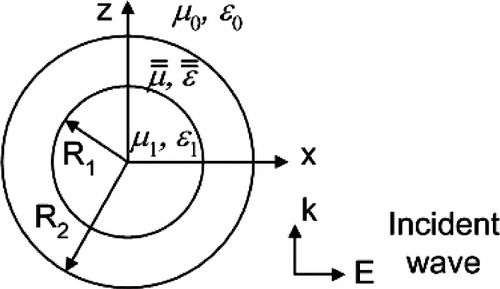
\includegraphics[height=0.25\paperheight]{fig1.png}
  \caption{}
  \label{fig:1}
\end{figure}

\begin{figure}[h]
  \centering
  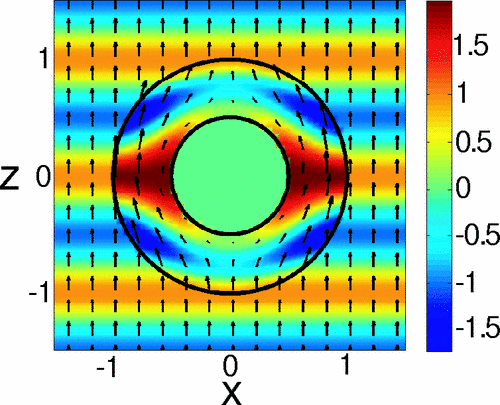
\includegraphics[height=0.25\paperheight]{fig2.png}
  \caption{}
  \label{fig:2}
\end{figure}

\begin{figure}[h]
  \centering
  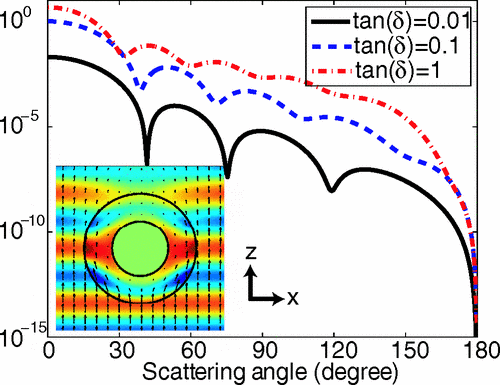
\includegraphics[height=0.3\paperheight]{fig3.png}
  \caption{}
  \label{fig:3}
\end{figure}

\begin{figure}[h]
  \centering
  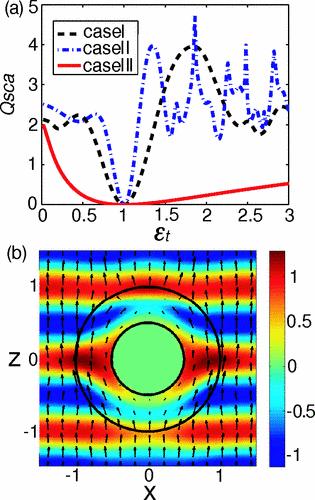
\includegraphics[height=0.4\paperheight]{fig4.png}
  \caption{}
  \label{fig:4}
\end{figure}
\end{document}
